% Source: Code/FLIR_Python/architecture_diagrams/system_architecture_simple.tex
\documentclass[border=10pt]{standalone}
\usepackage{tikz}
\usepackage{xcolor}
\usetikzlibrary{shapes.geometric, arrows.meta, positioning, fit, backgrounds, calc}

% USC Color Definitions
\definecolor{uscgarnet}{HTML}{73000a}
\definecolor{uscatlantic}{HTML}{466A9F}
\definecolor{usccongaree}{HTML}{1F414D}
\definecolor{uschorseshoe}{HTML}{65780B}
\definecolor{uscrose}{HTML}{CC2E40}
\definecolor{uscsandstorm}{HTML}{FFF2E3}
\definecolor{uscwarmgrey}{HTML}{676156}

\begin{document}

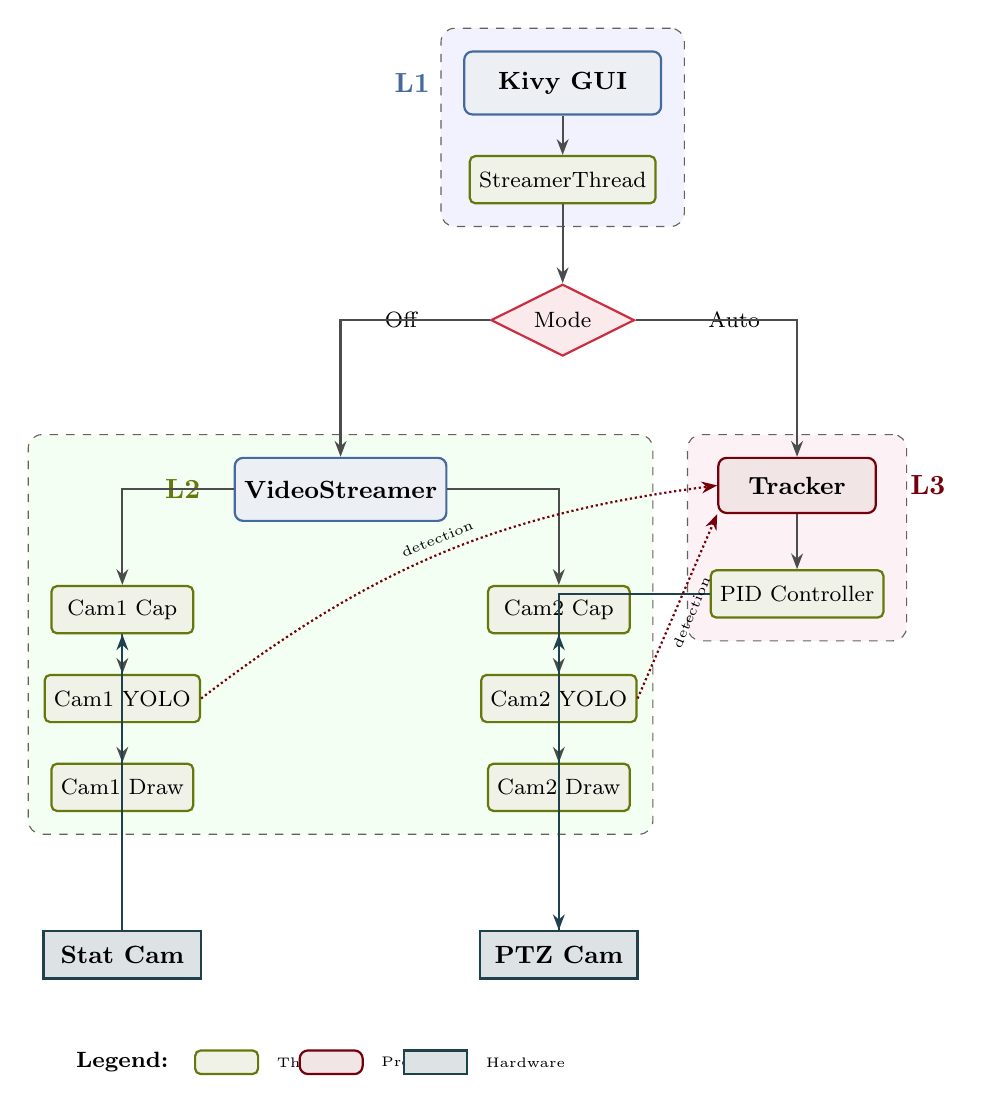
\begin{tikzpicture}[
    % Node styles (USC Colors)
    app/.style={rectangle, draw=uscatlantic, fill=uscatlantic!10, thick, minimum width=2.5cm, minimum height=0.8cm, align=center, rounded corners=3pt, font=\small\bfseries},
    thread/.style={rectangle, draw=uschorseshoe, fill=uschorseshoe!10, thick, minimum width=1.8cm, minimum height=0.6cm, align=center, rounded corners=2pt, font=\footnotesize},
    process/.style={rectangle, draw=uscgarnet, fill=uscgarnet!10, thick, minimum width=2cm, minimum height=0.7cm, align=center, rounded corners=3pt, font=\small\bfseries},
    hardware/.style={rectangle, draw=usccongaree, fill=usccongaree!15, thick, minimum width=2cm, minimum height=0.6cm, align=center, font=\small\bfseries},
    state/.style={rectangle, draw=uscrose, fill=uscrose!10, thick, minimum width=1.5cm, minimum height=0.5cm, align=center, font=\footnotesize\bfseries},
    decision/.style={diamond, draw=uscrose, fill=uscrose!10, thick, aspect=2, align=center, font=\footnotesize},
    container/.style={draw=uscwarmgrey, dashed, rounded corners=5pt, inner sep=8pt},
    % Arrow styles
    dataarrow/.style={-{Stealth[length=2mm]}, thick, draw=black!70},
    ipc/.style={-{Stealth[length=2mm]}, thick, draw=uscgarnet, densely dotted},
    hwlink/.style={-{Stealth[length=2mm]}, thick, draw=usccongaree},
]

% ============================================================================
% LAYER 1: GUI (Top)
% ============================================================================
\node[app] (gui) {Kivy GUI};
\node[thread, below=0.5cm of gui] (streamer) {StreamerThread};

% L1 label
\node[left=0.3cm of gui, font=\bfseries\color{uscatlantic}] {L1};

% Container for L1
\begin{scope}[on background layer]
    \node[container, fill=blue!5, fit=(gui)(streamer)] (l1box) {};
\end{scope}

% ============================================================================
% Mode Switch
% ============================================================================
\node[decision, below=1cm of streamer] (mode) {Mode};
\node[left=0.8cm of mode, font=\footnotesize] {Off};
\node[right=0.8cm of mode, font=\footnotesize] {Auto};

\draw[dataarrow] (gui) -- (streamer);
\draw[dataarrow] (streamer) -- (mode);

% ============================================================================
% LAYER 2: VideoStreamer (Left side)
% ============================================================================
\node[app, below left=1.5cm and 1cm of mode] (videostreamer) {VideoStreamer};

% Camera 1 Pipeline
\node[thread, below left=0.8cm and 0.5cm of videostreamer] (cam1cap) {Cam1 Cap};
\node[thread, below=0.5cm of cam1cap] (cam1yolo) {Cam1 YOLO};
\node[thread, below=0.5cm of cam1yolo] (cam1draw) {Cam1 Draw};

% Camera 2 Pipeline
\node[thread, below right=0.8cm and 0.5cm of videostreamer] (cam2cap) {Cam2 Cap};
\node[thread, below=0.5cm of cam2cap] (cam2yolo) {Cam2 YOLO};
\node[thread, below=0.5cm of cam2yolo] (cam2draw) {Cam2 Draw};

% L2 label
\node[left=0.3cm of videostreamer, font=\bfseries\color{uschorseshoe}] {L2};

% Container for L2
\begin{scope}[on background layer]
    \node[container, fill=green!5, fit=(videostreamer)(cam1cap)(cam1draw)(cam2cap)(cam2draw)] (l2box) {};
\end{scope}

% L2 internal connections
\draw[dataarrow] (videostreamer) -| (cam1cap);
\draw[dataarrow] (videostreamer) -| (cam2cap);
\draw[dataarrow] (cam1cap) -- (cam1yolo);
\draw[dataarrow] (cam1yolo) -- (cam1draw);
\draw[dataarrow] (cam2cap) -- (cam2yolo);
\draw[dataarrow] (cam2yolo) -- (cam2draw);

% Mode to VideoStreamer
\draw[dataarrow] (mode) -| node[above left, font=\tiny, pos=0.3] {} (videostreamer);

% ============================================================================
% LAYER 3: Tracker Process (Right side)
% ============================================================================
\node[process, below right=1.5cm and 1.5cm of mode] (tracker) {Tracker};
\node[thread, below=0.7cm of tracker] (pid) {PID Controller};

% L3 label
\node[right=0.3cm of tracker, font=\bfseries\color{uscgarnet}] {L3};

% Container for L3
\begin{scope}[on background layer]
    \node[container, fill=purple!5, fit=(tracker)(pid)] (l3box) {};
\end{scope}

% Mode to Tracker
\draw[dataarrow] (mode) -| node[above right, font=\tiny, pos=0.3] {} (tracker);

% Internal tracker flow
\draw[dataarrow] (tracker) -- (pid);

% ============================================================================
% LAYER 4: Hardware (Bottom)
% ============================================================================
\node[hardware, below=1.5cm of cam1draw] (statcam) {Stat Cam};
\node[hardware, below=1.5cm of cam2draw] (ptzcam) {PTZ Cam};

% Hardware connections
\draw[hwlink] (statcam) -- (cam1cap);
\draw[hwlink] (ptzcam) -- (cam2cap);
\draw[hwlink] (pid) -| (ptzcam);

% ============================================================================
% KEY TRACKING FLOW CONNECTIONS
% ============================================================================

% Cam1 YOLO --"detection"--> Tracker (coarse acquisition)
\draw[ipc, bend left=15] (cam1yolo.east) to node[above, font=\tiny, sloped] {detection} (tracker.west);

% Cam2 YOLO --"detection"--> Tracker (fine tracking)
\draw[ipc] (cam2yolo.east) to node[below, font=\tiny, sloped] {detection} (tracker.south west);

% Tracker --"redirect"--> PTZ Cam (via PID)
% Already shown via pid -> ptzcam

% ============================================================================
% Legend
% ============================================================================
\node[below=0.8cm of statcam, font=\footnotesize\bfseries] (legend) {Legend:};
\node[thread, right=0.2cm of legend, minimum width=0.8cm, minimum height=0.3cm] (lt) {};
\node[right=0.1cm of lt, font=\tiny] {Thread};
\node[process, right=0.5cm of lt, minimum width=0.8cm, minimum height=0.3cm] (lp) {};
\node[right=0.1cm of lp, font=\tiny] {Process};
\node[hardware, right=0.5cm of lp, minimum width=0.8cm, minimum height=0.3cm] (lh) {};
\node[right=0.1cm of lh, font=\tiny] {Hardware};

\end{tikzpicture}

\end{document}
